\chapter{GENERAL REVIEW OF LITERATURE}

\subsection{What are Grammars?}

Grammars in computer science can be defined as a set of rules by which valid sentences in a language are constructed \cite{jiangFormalGrammarsLanguages}, serving as a blueprint for the language. Beginning with a start symbol, which is a single non-terminal, production rules are applied sequentially, adding symbols from the alphabet according to the grammar’s production rules, to derive a string that is valid in the language \cite{GrammarTheoryComputation2025}.

\vspace{\baselineskip}

A grammar can be represented by the tuple $<N, T, P, S>$, where:
\begin{itemize}
\item $N$ is a finite, non-empty set of non-terminal symbols/alphabet.
\item $T$ is a finite set of terminal symbols/alphabet.
\item $P$ is a finite set of production rules.
\item $S$ is the start symbol (a non-terminal symbol/alphabet).
\end{itemize}

Here, the production rules $P$ define all symbol substitutions that can be performed recursively to generate different symbol sequences, known as \emph{strings} \cite{GrammarTheoryComputation2025}. These rules are written in the form $A \rightarrow w$, where $A \in N$ and $w \in (N \cup T)^*$.

\subsection{What are Context-Free Grammars?}

Depending on the set of production rules, each grammar can be classified according to the \emph{Chomsky hierarchy} \cite{chomskyTHREEMODELSTIE1956}.

\begin{center}
    \includegraphics[width=0.7\textwidth]{chapter1/ch_heir.png}
    \captionof{figure}{Chomsky hierarchy \cite{ChomskyHierarchyTheory2025}}
    \label{fig:hierarchy}
\end{center}

The hierarchy outlines four distinct types of grammars, ranging from \textbf{Type-3} (the most restrictive) to \textbf{Type-0} (the most general and unstructured). \textbf{Type-2} grammars in this hierarchy are known as \emph{context-free grammars}.

\subsubsection{Type-3}
Type-3 grammars, known as regular grammars are used to generate regular languages. A grammar is classified as a regular grammar if its production rules follow from $X \rightarrow a | X \rightarrow aY$. The left-hand side must consist of a single $T$ and the right-hand side must consist of an single $T$ or single $T$ and single $N$.

Regular grammar can take 2 froms, right linear and left linear.

Right-linear take the following form, where the $N$ on the right-hand side of the arrow is on the far right.
\begin{itemize}
    \item[] $X \rightarrow a$
    \item[] $X \rightarrow aB$
    \item[] $X \rightarrow \varepsilon$
\end{itemize}

Left-linear take the following form, where the $N$ on the right-hand side of the arrow is on the far left.
\begin{itemize}
    \item[] $X \rightarrow a$
    \item[] $X \rightarrow Ba$
    \item[] $X \rightarrow \varepsilon$
\end{itemize}

Note that right-linear and left-linear forms cannot be mixed, 
as doing so may generate languages that are not regular. 
Additionally, production of $\varepsilon$ is allowed only if the corresponding nonterminal 
does not appear on the right-hand side of any production rule \cite{hendriksConsiderItParsed,shiIntelligenceScience2021}

\subsubsection{Type-2}

Type-2 grammars, commonly known as context-free grammars, have production rules of the form:
\[
A \rightarrow \alpha
\]
where \( A \in N \) and \( \alpha \in (T \cup N)^* \), meaning any string composed of terminal and nonterminal symbols \cite{hendriksConsiderItParsed,shiIntelligenceScience2021}.

Due to the nature of the right-hand side, nonterminals are allowed to recursively expand, which can lead to repetition. For example:
\begin{itemize}
    \item[] \( A \rightarrow sAb \)
    \item[] \( A \rightarrow \varepsilon \)
\end{itemize}
can produce derivations of the form
\[
A \Rightarrow sAb \Rightarrow ssAbb \Rightarrow \cdots \Rightarrow s^n b^n,
\]
until eventually \( A \Rightarrow \varepsilon \).

This property is particularly useful because it allows the grammar to enforce well-formed parenthesis expressions and other recursive structures purely through production rules. As a result, context-free grammars are of great importance in the design and specification of programming languages\cite{hendriksConsiderItParsed,shiIntelligenceScience2021}.

\subsubsection{Type-1}

Type-1 grammars, also known as context-sensitive grammars, have production rules of the form:
\[
\alpha A \beta \rightarrow \alpha \gamma \beta
\]
where \( A \in N \) and \( \alpha, \beta, \gamma \in (N \cup T)^* \). This means that \( A \) can be expanded to \( \gamma \) only in the specific context where it appears between \( \alpha \) and \( \beta \) in the given order \cite{hendriksConsiderItParsed,shiIntelligenceScience2021}.

\vspace{\baselineskip}
A key property of context-sensitive grammars is that production rules must be \emph{non-contracting}: the length of the right-hand side must be greater than or equal to the length of the left-hand side. This implies that no nonterminal on the right-hand side can derive \( \varepsilon \), meaning nullable productions are not allowed.

An example derivation using a context-sensitive production is:
\[
A \Rightarrow aA\beta \Rightarrow aaA\beta\beta \Rightarrow \cdots
\]

\subsubsection{Type-0}

Type-0 grammars, also known as unrestricted grammars, sit at the top of Chomsky's hierarchy. Their production have a complete lack of restrictions and take the general form:
\[
\alpha \rightarrow \beta
\]
where \( \alpha, \beta \in (N \cup T)^+ \), meaning they are strings consisting of terminal and nonterminal symbols. The only requirement is that \( \alpha \) must contain at least one nonterminal symbol to allow for further derivations \cite{hendriksConsiderItParsed,shiIntelligenceScience2021}.

Type-0 grammars are the most expressive class in the Chomsky hierarchy and can generate all recursively enumerable languages.

\subsection{What is ARVADA?}

\subsubsection{Introduction}

ARVADA is an algorithm published in \enquote{Learning Highly Recursive Input Grammars} \cite{kulkarniLearningHighlyRecursive2021} at the University of California, Berkeley in 2021. It is designed to learn context-free grammars from a set of positive examples and a Boolean-valued oracle $\mathcal{O}$. Starting from initially flat parse trees, ARVADA repeatedly applies two specialized operations, \textbf{bubbling} and \textbf{merging}, to incrementally add structure to these trees. From this structured representation, it extracts the smallest possible set of context-free grammar rules that accommodate all the given examples. The algorithm aims to generalize the language as much as possible without overgeneralizing beyond what is accepted by $\mathcal{O}$.

\vspace{\baselineskip}
Like GLADE \cite{bastaniSynthesizingProgramInput}, ARVADA operates under the assumption of a black-box oracle $\mathcal{O}$. This means that ARVADA has no access to or knowledge of the internal workings of the oracle and can only observe the Boolean values returned by $\mathcal{O}$.

\subsubsection{Explanation}

ARVADA takes as input the oracle $\mathcal{O}$ and a set of positive, valid oracle inputs $S$. For each string $s \in S$, querying $\mathcal{O}(s)$ returns \verb|True|. The algorithm begins by constructing a flat parse tree for each string in $S$. Each tree has a single root node $t_0$ whose children correspond to the individual characters of the input string $s$.

\vspace{\baselineskip}
Next, ARVADA performs the \textbf{bubbling} operation. In this step, a sequence of sibling nodes in the tree is selected and replaced with a new non-terminal node. This new node takes the selected sibling nodes as its children, thereby introducing an additional level of structure. Essentially, ARVADA transforms sequences of terminal nodes in the flat parse tree into subtrees by introducing new non-terminal nodes and progressively adding structure to the tree.

\vspace{\baselineskip}
ARVADA then decides whether to accept or reject each bubble by checking whether the newly bubbled structure enables a sound generalization of the learned grammar. Each non-leaf node in the tree can be viewed as a non-terminal in the emerging grammar. To determine whether a bubble should be accepted, ARVADA checks whether replacing any node in the tree with the new bubbled subtree results in the generation of valid input strings according to $\mathcal{O}$. If the replacement produces valid strings, the bubble is accepted, and the tree is restructured so that both the bubbled subtree and the replaced node share the same non-terminal label.

\vspace{\baselineskip}
The addition of new non-terminal nodes expands the language defined by the learned grammar, since any string derivable from the same label can now be substituted interchangeably. This relabeling of the bubbled subtree and the replaced node is called a \textbf{merge}, as it merges the labels of two previously distinct nodes in the tree. If a bubble is not accepted, it is discarded, and none of the trees are affected or structurally modified.

\subsubsection{Walkthrough}

This walkthorugh will follow very closely to the examples provided in the original paper \cite{kulkarniLearningHighlyRecursive2021}, and use a concrete example to provide an indepth understanding of ARVADA.

%%%%%%%%% GRAMMAR %%%%%%%%%%%
\begin{figure}[H]
\begin{tcolorbox}[title=$G_w$, colback=white, colframe=black]
\begin{grammar}{
    \pr{\emph{start}}{\emph{stmt}}
    
    \pr{\emph{stmt}}{while\textvisiblespace\ \emph{boolexpr}\textvisiblespace\ do\textvisiblespace\ \emph{stmt}}
    & & \gors if\textvisiblespace\ \emph{boolexpr}\textvisiblespace\ then\textvisiblespace\ \emph{stmt}\textvisiblespace\ else\textvisiblespace\ \emph{stmt}\\
    & & \gors L\textvisiblespace\ =\textvisiblespace\ \emph{numexpr}\\
    & & \gors \emph{stmt}\textvisiblespace\ ;\textvisiblespace\ \emph{stmt}\\
    
    \pr{\emph{boolexpr}}{$\thicksim$\emph{boolexpr}}
    & & \gors \emph{boolexpr}\textvisiblespace\ \&\textvisiblespace\ \emph{boolexpr}\\
    & & \gors \emph{numexpr}\textvisiblespace\ ==\textvisiblespace\ \emph{numexpr}\\
    & & \gors false\\
    & & \gors true\\
    
    \pr{\emph{numexpr}}{(\textvisiblespace\ \emph{numexpr}\textvisiblespace\ +\textvisiblespace\ \emph{numexpr}\textvisiblespace\ )}
    & & \gors L\\
    & & \gors n\\
}
\end{grammar}
\end{tcolorbox}

\[
S = \left\{
\text{\texttt{while true \& false do L = n}},
\quad
\text{\texttt{L = n ; L = (n+n)}}
\right\}
\]

\[
O(i) =
\begin{cases}
\text{True} & \text{if } i \in \mathcal{L}(G_w) \\
\text{False} & \text{otherwise}
\end{cases}
\]
\caption{Definition a simple while grammar $G_w$, sample input strings $S$, and oracle $\mathcal{O}$ \cite{kulkarniLearningHighlyRecursive2021}}
\label{fig:grammar}
\end{figure}
%%%%%%%%%%%%%%%%%%%

%%% proof read here please %%%%%
For this walkthrough, the simple while grammar $G_w$ and input string $S$ provided in figure~\ref{fig:grammar} will be used. Noting agian that ARVADA treats $\mathcal{O}$ as a blackbox, meaning it has no sturcture knowledge of $G_w$, and $G_w$ in only shown to clarify the behaviour of $\mathcal{O}$.

%%%%% Pseudocode $$$$$$
\begin{algorithm}[H]
\caption{High-level overview of ARVADA \cite{kulkarniLearningHighlyRecursive2021}}\label{alg:arv}
\begin{algorithmic}[1]
    \Require a set of examples $S$, a language oracle $\mathcal{O}$.
    \State $bestTrees \gets \textsc{NaiveParseTrees}(S)$
    \State $bestTrees \gets \textsc{MergeAllValid}(bestTrees, \mathcal{O})$
    \State $updated \gets \text{True}$
    \While{$updated$}
        \State $updated \gets \text{False}$
        \State $allBubbles \gets \textsc{GetBubbles}(bestTrees)$
        \For{$bubble$ \textbf{in} $allBubbles$}
            \State $bbldTrees \gets \textsc{Apply}(bestTrees, bubble)$
            \State $accepted, mergedTs \gets \textsc{CheckBubble}(bbldTrees, \mathcal{O})$
            \If{$accepted$}
                \State $bestTrees \gets mergedTs$
                \State $updated \gets \text{True}$
                \State \textbf{break}
            \EndIf
        \EndFor
    \EndWhile
    \State $G \gets \textsc{InducedGrammar}(bestTrees)$
    \State \textbf{Return} $G$
\end{algorithmic}
\end{algorithm}

ARVADA follows the high-level overview provided in algorithm ~\ref{alg:arv}, and begin by taking the all the inputs string in $S$ and building naive flat parse tree for each input stirng.

\begin{figure}[h!]
\centering
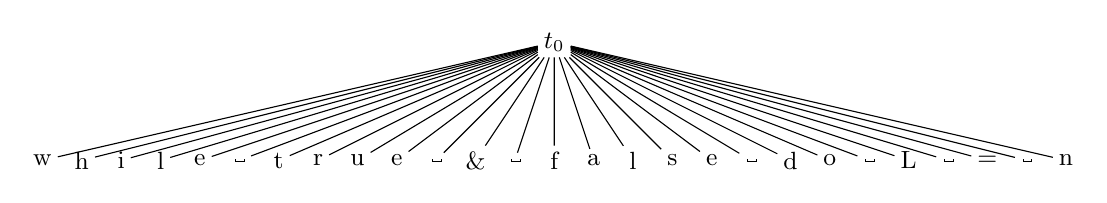
\begin{tikzpicture}[
    level distance=15mm,
    sibling distance=5mm,
    every node/.style={draw=none, inner sep=2pt, font=\small},
    edge from parent/.style={draw}
]
    \node {$t_0$}
        child {node {w}}
        child {node {h}}
        child {node {i}}
        child {node {l}}
        child {node {e}}
        child {node {\textvisiblespace}}
        child {node {t}}
        child {node {r}}
        child {node {u}}
        child {node {e}}
        child {node {\textvisiblespace}}
        child {node {\&}}
        child {node {\textvisiblespace}}
        child {node {f}}
        child {node {a}}
        child {node {l}}
        child {node {s}}
        child {node {e}}
        child {node {\textvisiblespace}}
        child {node {d}}
        child {node {o}}
        child {node {\textvisiblespace}}
        child {node {L}}
        child {node {\textvisiblespace}}
        child {node {=}}
        child {node {\textvisiblespace}}
        child {node {n}};
\end{tikzpicture}

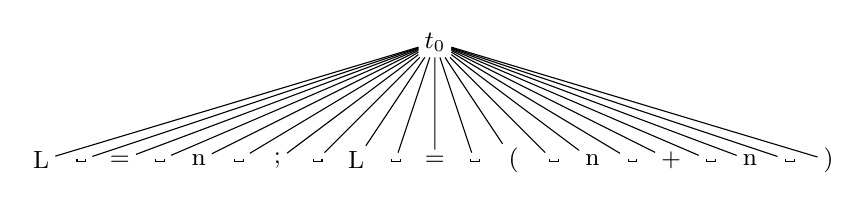
\begin{tikzpicture}[
    level distance=15mm,
    sibling distance=5mm,
    every node/.style={draw=none, inner sep=2pt, font=\small},
    edge from parent/.style={draw}
]
\node {$t_0$}
    child {node {L}}
    child {node {\textvisiblespace}}
    child {node {=}}
    child {node {\textvisiblespace}}
    child {node {n}}
    child {node {\textvisiblespace}}
    child {node {;}}
    child {node {\textvisiblespace}}
    child {node {L}}
    child {node {\textvisiblespace}}
    child {node {=}}
    child {node {\textvisiblespace}}
    child {node {(}}
    child {node {\textvisiblespace}}
    child {node {n}}
    child {node {\textvisiblespace}}
    child {node {+}}
    child {node {\textvisiblespace}}
    child {node {n}}
    child {node {\textvisiblespace}}
    child {node {)}};    
\end{tikzpicture}
\caption{Initial set of flat naive prase trees ARVADA builds given inputs $S$, where each $t_i$ is a non-terminal}
\label{fig:initialNaiveTrees}
\end{figure}

The Naive parse trees initially built by ARVDA for input set $S$ shown in figure \ref{fig:initialNaiveTrees}.

\[
t_0 \to \text{w\;h\;i\;l\;e\;\textvisiblespace\;t\;r\;u\;e\textvisiblespace\&\;f\;a\;l\;s\;e\;\textvisiblespace\;d\;o\;\textvisiblespace\;L\;\textvisiblespace=\;\textvisiblespace\;n}
\]
\[
t_0 \to \text{L\;\textvisiblespace\;=\;\textvisiblespace \;n\;\textvisiblespace\;;\;\textvisiblespace\;L\;\textvisiblespace\;=\;\textvisiblespace\;(\;n\;+\;n\;)}
\]

\subsection{Why C?}

In the original study \cite{kulkarniLearningHighlyRecursive2021}, the ARVADA algorithm was implemented in Python. When compared to GLADE \cite{bastaniSynthesizingProgramInput}, which was implemented in Java, ARVADA exhibited a slower average runtime across all benchmarks. In the study, this was attributed to the natural runtime disadvantage of Python compared to Java, which is valid, however the possibility that ARVADA itself might be inherently slow was not acknowledged.

\vspace{\baselineskip}

In a comparative study, A Pragmatic Comparison of Four Different Programming Languages \cite{aliPragmaticComparisonFour2021}, it was found that when speed and efficiency are prioritized, C is a better choice than Python. As a mid-level, statically typed, and structured language that runs under a compiler, C consistently outperforms dynamically typed, interpreted languages such as Python \cite{kumarPythonLanguageComparison2022}. Moreover, C’s provision of only essential features contributes to its efficiency but also increases programming complexity compared to Python \cite{aliPragmaticComparisonFour2021, kumarPythonLanguageComparison2022}.

\vspace{\baselineskip}

Therefore, to investigate and potentially address runtime bottlenecks, C was selected as the implementation language for this replication study. The added complexity inherent to programming in C, relative to Python, was also acknowledged.

\subsection{Why replicate ARVADA?}
The replication study of GLADE \cite{bastaniSynthesizingProgramInput} conducted by researchers at CISPA \cite{bendrissouSynthesizingInputGrammars2022} in 2022 reported results that were inconsistent with those presented in the original paper \cite{bastaniSynthesizingProgramInput}. Since ARVADA is closely related to GLADE, sharing a similar purpose and experimental setting, there is reason to suspect that ARVADA may also yield inconsistent results upon reimplementation.

\vspace{\baselineskip}

Another motivation for replication arises from the incomplete nature of the ARVADA study and its evaluation. Although the paper presents a reasonable amount of testing and statistical data, compares the algorithm with GLADE, and provides a detailed explanation of ARVADA, it does not offer formal guarantees. It remains unclear whether ARVADA is applicable in all scenarios or what subset of scenarios it can reliably handle. Furthermore, when comparing ARVADA with GLADE, there is a possibility that the grammars used for testing were selected based on performance considerations, raising suspicions that the study may have been selective.

\subsection{Why is learning highly input grammar important?}
incldue what are parser.
Software in the modern world is abundant, ranging in size, function, and use. Although abundant, due to privacy and security laws around the world, accessing the sources code of many of these software and programs have become impossible. Hence, the importance recursive input grammars. Treating the program as a Blackbox and recursively using input grammar against it to reverse engineer the grammar of the program to help with program comprehension and understanding.   

\subsection{Related Work}
\subsubsection{GLADE}
GLADE is an algorithm proposed by Bastani et al., published in Synthesizing Input Grammars at PLDI 2017 \cite{bastaniSynthesizingProgramInput}. Like ARVADA, GLADE uses a set of valid inputs and black-box access to the program, with the aim of automatically approximating the context-free input grammar of the given program.

\vspace{\baselineskip}

Because GLADE and ARVADA share a similar experimental setting, GLADE was used as a benchmark for ARVADA during its evaluation. It was shown that GLADE, on average, had a faster runtime compared to ARVADA. However in terms of generalization, following the original grammar of the oracle more closely, ARVADA out-performed GLADE across the 11 benchmarks, achieving a higher F1 score on 9 of the 11 benchmarks.


What are similar work, and progression done in this field since the publication of ARVADA? 

\subsection{Problem Statement}

Due to the unknowns and gaps in the original paper \cite{kulkarniLearningHighlyRecursive2021}—including the lack of guarantees regarding the kinds of grammars ARVADA can handle and the complexity of the grammars it can learn—along with the suspicion that the original study may have been selective in nature, this thesis aims to achieve the following:

\vspace{\baselineskip}
A replication of the study “Learning Highly Recursive Input Grammars” \cite{kulkarniLearningHighlyRecursive2021}, through a clean-room re-implementation of ARVADA, with the intention of expanding its evaluation to include a wider variety of grammars and identifying its key characteristics.

\vspace{\baselineskip}
The clean-room re-implementation will mean development is entirely from scratch in a new environment, based solely on the explanations provided in the original paper. This will also enable for an assessment of the adequacy of those explanations—specifically, whether a complete re-implementation is possible based on the information given or if the paper lacks essential details for reproducability.

\vspace{\baselineskip}
Although the primary goal of this study is to re-implemention, assessment, and expantion upon the original work, I acknowledge that this study may be incomplete or no new knowledge may be discovered. While this may seem trivial—merely confirming the findings of the previous study without adding novel insights \cite{hendriksConsiderItParsed}, replication studies play a vital role in reinforcing the trustworthiness and confidence of empirical results, which is a central tent of the scientific method. Replication can increase certainty when findings are reproduce and promote innovation when they are not \cite{shepperdReplicationStudiesConsidered2018}. Therefore, this study holds significance within the field of computer science.



